\documentclass[aspectratio=169,11pt,xcolor=table]{beamer}

% ==============================================================================
% PAQUETES
% ==============================================================================
\usepackage[utf8]{inputenc}
\usepackage[T1]{fontenc}
\usepackage[spanish,es-tabla,es-nodecimaldot]{babel}
\usepackage{lmodern}
\usepackage{graphicx}
\usepackage{booktabs}
\usepackage{array}
\usepackage{amsmath,amssymb}
\usepackage{fontawesome5}
\usepackage[most]{tcolorbox}
\usepackage{tikz}
\usetikzlibrary{arrows.meta,positioning,shapes.geometric,calc,backgrounds}
\usepackage{hyperref}

% ==============================================================================
% DISEÑO VISUAL (Guía: 2-3 colores principales, fondo claro, alto contraste)
% ==============================================================================
\definecolor{bglight}{HTML}{FFFFFF}      % Fondo blanco puro (mucho espacio en blanco)
\definecolor{bgsoft}{HTML}{F1F5F9}       % Gris muy suave para tarjetas puntuales
\definecolor{inkdark}{HTML}{0F172A}      % Texto oscuro de alto contraste
\definecolor{inkmuted}{HTML}{475569}     % Texto secundario
\definecolor{brandblue}{HTML}{1D4ED8}    % Color principal 1: Azul Ingeniería
\definecolor{brandgreen}{HTML}{059669}   % Color principal 2: Verde Esmeralda
\definecolor{brandamber}{HTML}{D97706}   % Color de apoyo: Ámbar

\setbeamertemplate{navigation symbols}{}
\setbeamercolor{background canvas}{bg=bglight}
\setbeamercolor{normal text}{fg=inkdark,bg=bglight}
\setbeamercolor{structure}{fg=brandblue}
\setbeamercolor{frametitle}{fg=inkdark,bg=bglight}
\setbeamercolor{itemize item}{fg=brandblue}

\setbeamertemplate{itemize item}{\normalsize\raise0.5pt\hbox{\faCheckCircle}}

\tcbset{coltext=inkdark}

% Encabezado minimalista con aire pero compacto
\makeatletter
\setbeamertemplate{frametitle}{%
  \vspace{0.18cm}%
  \begin{beamercolorbox}[wd=\paperwidth,leftskip=0.6cm,rightskip=0.6cm]{frametitle}%
    {\large\bfseries\color{inkdark}\insertframetitle}%
    \ifx\insertframesubtitle\@empty\else%
      \\[2pt]{\footnotesize\color{brandblue}\textbf{\insertframesubtitle}}%
    \fi%
  \end{beamercolorbox}%
  \vspace{-0.08cm}%
  \hspace{0.6cm}{\color{brandblue}\rule{2.0cm}{1.6pt}}%
}
\makeatother

% Pie de página minimalista
\setbeamertemplate{footline}{%
  \begin{beamercolorbox}[wd=\paperwidth,ht=0.45cm,dp=0.16cm,leftskip=0.6cm,rightskip=0.6cm]{background canvas}%
    {\scriptsize\color{inkmuted}\textbf{\color{brandblue}\faBolt\ ARCEUS GRID}\quad|\quad Monitoreo Eléctrico \& AIoT}
    \hfill
    {\scriptsize\color{inkmuted}\textbf{\color{inkdark}\insertframenumber}\ / \insertmainframenumber}
  \end{beamercolorbox}%
}

% Tarjeta suave minimalista
\newtcolorbox{softcard}[2][brandblue]{%
  enhanced,
  colback=bgsoft,
  colframe=bgsoft,
  borderline west={3pt}{0pt}{#1},
  boxrule=0pt,
  arc=4pt,
  left=8pt,right=8pt,top=5pt,bottom=5pt,
  boxsep=2pt,
  fonttitle=\bfseries\small,
  coltitle=#1,
  colbacktitle=bgsoft,
  title={#2}
}

\begin{document}

% ==============================================================================
% 1. PORTADA (Guía: Título claro, ilustración/icono atractivo, autor y fecha)
% ==============================================================================
\begin{frame}[plain]
  \begin{tikzpicture}[remember picture,overlay]
    \fill[brandblue!12] (current page.north west) -- ++(4.2,0) -- ++(-4.2,-2.6) -- cycle;
    \fill[brandgreen!12] (current page.south east) -- ++(-4.5,0) -- ++(4.5,2.8) -- cycle;
    \fill[brandamber!15] ($(current page.north east)+(-2.2,-1.1)$) circle (0.9cm);
    \fill[brandblue!10] ($(current page.south west)+(2.0,1.0)$) circle (0.7cm);
  \end{tikzpicture}

  \vspace{1.2cm}
  \begin{center}
    {\Large\color{brandblue}\faBolt\quad\faMicrochip\quad\faBrain}\\[10pt]
    {\Huge\bfseries\color{inkdark}ARCEUS GRID}\\[10pt]
    {\large\color{inkmuted}Monitoreo Eléctrico 12V DC, ESP-NOW y Aprendizaje Federado}\\[16pt]
    \begin{tikzpicture}
      \node[fill=brandgreen!15,draw=brandgreen,line width=0.9pt,rounded corners=4pt,
            inner xsep=14pt,inner ysep=7pt,align=center,font=\small\bfseries,text=inkdark]
        {Owen Mora $\cdot$ Angelo Charris $\cdot$ Braulio Ribón\\[2pt]
         Manuel Pertuz $\cdot$ Milton Sánchez};
    \end{tikzpicture}
  \end{center}
\end{frame}

% ==============================================================================
% 2. CONTENIDO / ESTRUCTURA (Guía: Tarjetas limpias de Inicio - Desarrollo - Cierre)
% ==============================================================================
\begin{frame}{Contenido de la Presentación}{Estructura: Inicio $\cdot$ Desarrollo $\cdot$ Cierre}
  \vspace{0.1cm}
  \begin{columns}[T,onlytextwidth]
    \begin{column}{0.31\textwidth}
      \begin{tcolorbox}[colback=brandblue!10,colframe=brandblue!40,boxrule=0.7pt,arc=4pt,halign=center,top=4pt,bottom=4pt,boxsep=1pt]
        {\large\color{brandblue}\faExclamationTriangle}\\[2pt]
        {\small\bfseries 1. El Problema}\\[1pt]
        {\scriptsize Riesgos en 12V DC y nube}
      \end{tcolorbox}
      \vspace{0.12cm}
      \begin{tcolorbox}[colback=brandgreen!10,colframe=brandgreen!40,boxrule=0.7pt,arc=4pt,halign=center,top=4pt,bottom=4pt,boxsep=1pt]
        {\large\color{brandgreen}\faLock}\\[2pt]
        {\small\bfseries 4. Hardware Seguro}\\[1pt]
        {\scriptsize Aislamiento JD-VCC y Star GND}
      \end{tcolorbox}
    \end{column}

    \begin{column}{0.31\textwidth}
      \begin{tcolorbox}[colback=brandgreen!10,colframe=brandgreen!40,boxrule=0.7pt,arc=4pt,halign=center,top=4pt,bottom=4pt,boxsep=1pt]
        {\large\color{brandgreen}\faLayerGroup}\\[2pt]
        {\small\bfseries 2. La Solución}\\[1pt]
        {\scriptsize Plataforma en 3 niveles}
      \end{tcolorbox}
      \vspace{0.12cm}
      \begin{tcolorbox}[colback=brandamber!12,colframe=brandamber!50,boxrule=0.7pt,arc=4pt,halign=center,top=4pt,bottom=4pt,boxsep=1pt]
        {\large\color{brandamber}\faBroadcastTower}\\[2pt]
        {\small\bfseries 5. Red ESP-NOW}\\[1pt]
        {\scriptsize INA219 + ESP-NOW + MQTT}
      \end{tcolorbox}
    \end{column}

    \begin{column}{0.31\textwidth}
      \begin{tcolorbox}[colback=brandamber!12,colframe=brandamber!50,boxrule=0.7pt,arc=4pt,halign=center,top=4pt,bottom=4pt,boxsep=1pt]
        {\large\color{brandamber}\faServer}\\[2pt]
        {\small\bfseries 3. Hardware Físico}\\[1pt]
        {\scriptsize 2 Estaciones + 1 Gateway}
      \end{tcolorbox}
      \vspace{0.12cm}
      \begin{tcolorbox}[colback=brandblue!10,colframe=brandblue!40,boxrule=0.7pt,arc=4pt,halign=center,top=4pt,bottom=4pt,boxsep=1pt]
        {\large\color{brandblue}\faBrain}\\[2pt]
        {\small\bfseries 6. IA y Resultados}\\[1pt]
        {\scriptsize Resultados e interfaz en vivo}
      \end{tcolorbox}
    \end{column}
  \end{columns}
\end{frame}

% ==============================================================================
% 3. PLANTEAMIENTO DEL PROBLEMA (Regla 6x6: 4 viñetas de <= 6 palabras + gráfico)
% ==============================================================================
\begin{frame}{1. El Problema en Microrredes}{¿Qué ocurre si una sobrecarga tarda en detectarse?}
  \vspace{0.15cm}
  \begin{columns}[c,onlytextwidth]
    \begin{column}{0.55\textwidth}
      \normalsize
      \begin{itemize}\setlength{\itemsep}{10pt}
        \item \textbf{Fusibles pasivos} sin telemetría en vivo.
        \item \textbf{Datos crudos} colapsan el Wi-Fi local.
        \item \textbf{Nube central} expone hábitos privados.
        \item \textbf{Ruido inductivo} reinicia los microcontroladores.
      \end{itemize}
    \end{column}
    \begin{column}{0.41\textwidth}
      \begin{softcard}[brandamber]{\faLightbulb\ Brecha Técnica}
        \small
        Se requiere \textbf{corte en milisegundos} en el borde y \textbf{aprendizaje predictivo} sin enviar datos crudos a internet.
      \end{softcard}
    \end{column}
  \end{columns}
\end{frame}

% ==============================================================================
% 4. LA SOLUCIÓN ARCEUS GRID (Regla 6x6 + Infografía simple de 3 bloques)
% ==============================================================================
\begin{frame}{2. La Solución: ARCEUS GRID}{Plataforma Ciberfísica Desacoplada en 3 Niveles}
  \vspace{0.1cm}
  \begin{columns}[c,onlytextwidth]
    \begin{column}{0.52\textwidth}
      \normalsize
      \begin{itemize}\setlength{\itemsep}{10pt}
        \item \textbf{Medición precisa} de $V, I, P$ (INA219).
        \item \textbf{Radio ESP-NOW} menor a $5\text{ ms}$.
        \item \textbf{Corte local} automático ($I > 1.80\text{ A}$).
        \item \textbf{IA FedAvg} con $100\%$ privacidad.
      \end{itemize}
    \end{column}
    \begin{column}{0.45\textwidth}
      \centering
      \begin{tikzpicture}[
        node distance=0.35cm,
        b/.style={draw=brandblue,fill=bgsoft,rounded corners=4pt,minimum width=4.9cm,minimum height=0.88cm,align=center,font=\scriptsize\bfseries,line width=0.85pt},
        ar/.style={-{Stealth[length=2.2mm]},line width=1.1pt,draw=brandblue}
      ]
        \node[b] (n1) {\color{brandblue}1. Borde: Estaciones A y B\\[-1pt]{\tiny\normalfont ESP32 + INA219 + Relés 12V}};
        \node[b,below=of n1,draw=brandamber] (n2) {\color{brandamber}2. Puente: Gateway Central\\[-1pt]{\tiny\normalfont Radio ESP-NOW (24 B) $\rightarrow$ MQTT}};
        \node[b,below=of n2,draw=brandgreen] (n3) {\color{brandgreen}3. Coordinador: Servidor Docker\\[-1pt]{\tiny\normalfont Mosquitto + SQLite WAL + FedAvg}};
        \draw[ar] (n1) -- (n2);
        \draw[ar] (n2) -- (n3);
      \end{tikzpicture}
    \end{column}
  \end{columns}
\end{frame}

% ==============================================================================
% 5. ARQUITECTURA FÍSICA (Guía: Resume datos complejos en una tabla limpia)
% ==============================================================================
\begin{frame}{3. Hardware Físico del Sistema}{Dos Estaciones Sensoras Autónomas y un Gateway}
  \vspace{0.15cm}
  \centering
  \small
  \renewcommand{\arraystretch}{1.42}
  \begin{tabular}{>{\bfseries\color{brandblue}}p{2.9cm} p{4.9cm} p{4.2cm}}
    \toprule
    \textbf{\color{inkdark}Módulo} & \textbf{\color{inkdark}Componentes Clave} & \textbf{\color{inkdark}Función Principal} \\
    \midrule
    Estación A & ESP32, INA219, OLED, 2 Bombillas & Censado y corte local \\
    \rowcolor{bgsoft}
    Estación B & ESP32, INA219, OLED, 2 Bombillas & Monitoreo de segunda rama \\
    Gateway Main & 1x ESP32 en Modo Dual & Traduce ESP-NOW a MQTT \\
    \rowcolor{bgsoft}
    Servidor Central & Docker, SQLite WAL, Streamlit & Dashboard y rondas FedAvg \\
    \bottomrule
  \end{tabular}
\end{frame}

% ==============================================================================
% 6. INGENIERÍA ELÉCTRICA Y SEGURIDAD (Regla 6x6 + Esquema limpio)
% ==============================================================================
\begin{frame}{4. Ingeniería de Hardware Seguro}{Cero Reinicios mediante Aislamiento Galvánico}
  \vspace{0.1cm}
  \begin{columns}[c,onlytextwidth]
    \begin{column}{0.53\textwidth}
      \normalsize
      \begin{itemize}\setlength{\itemsep}{10pt}
        \item \textbf{Relés aislados} sin jumper \texttt{JD-VCC}.
        \item \textbf{Optoacopladores} separan $3.3\text{ V}$ y $5\text{ V}$.
        \item \textbf{Tierra en estrella} elimina ruido analógico.
        \item \textbf{Buck LM2596} regula $12\text{ V}$ a $5.0\text{ V}$.
      \end{itemize}
    \end{column}
    \begin{column}{0.44\textwidth}
      \centering
      \begin{tikzpicture}[
        b/.style={draw=brandblue,fill=bgsoft,rounded corners=3pt,minimum width=4.5cm,minimum height=0.72cm,align=center,font=\scriptsize\bfseries,line width=0.85pt},
        ar/.style={-{Stealth[length=2mm]},line width=1pt,draw=brandgreen}
      ]
        \node[b] (f1) at (0,0) {Fuente Central 12V DC / 10A};
        \node[b,draw=brandamber] (f2) at (0,-1.05) {Regulador LM2596 ($12\text{ V} \rightarrow 5.0\text{ V}$)};
        \node[b,draw=brandgreen] (f3) at (0,-2.1) {Optoacoplador: Lógica $3.3\text{ V}$ $\parallel$ Bobina $5\text{ V}$};
        \node[b,draw=inkdark,fill=brandamber!15] (f4) at (0,-3.15) {$\bigstar$ Tierra en Estrella (Borne Único 0V)};
        \draw[ar] (f1) -- (f2);
        \draw[ar] (f2) -- (f3);
        \draw[ar] (f3) -- (f4);
      \end{tikzpicture}
    \end{column}
  \end{columns}
\end{frame}

% ==============================================================================
% 7. INSTRUMENTACIÓN: INA219 + OLED (Regla 6x6 + Tarjeta de Fórmula)
% ==============================================================================
\begin{frame}{5. Instrumentación: INA219 y OLED}{Medición High-Side en Tiempo Real sin Bloqueos}
  \vspace{0.15cm}
  \begin{columns}[c,onlytextwidth]
    \begin{column}{0.55\textwidth}
      \normalsize
      \begin{itemize}\setlength{\itemsep}{10pt}
        \item \textbf{Shunt $0.1\ \Omega$} en línea positiva $+12\text{ V}$.
        \item \textbf{Resolución fina} de $\pm 0.8\text{ mA}$ (12 bits).
        \item \textbf{Muestreo rápido} cada $200\text{ ms}$ ($400\text{ kHz}$).
        \item \textbf{Pantalla OLED} refrescada cada $300\text{ ms}$.
      \end{itemize}
    \end{column}
    \begin{column}{0.41\textwidth}
      \begin{softcard}[brandblue]{\faWaveSquare\ Ley de Medición Local}
        \centering\small
        \[
          I = \frac{V_{\text{shunt}}}{0.1\ \Omega}, \qquad P = V_{\text{bus}} \times I
        \]
        {\scriptsize\color{inkmuted}Multitarea cooperativa con \texttt{millis()}}
      \end{softcard}
    \end{column}
  \end{columns}
\end{frame}

% ==============================================================================
% 8. COMUNICACIONES: ESP-NOW + MQTT (Regla 6x6 + Comparativa Visual)
% ==============================================================================
\begin{frame}{6. Red Híbrida: ESP-NOW + MQTT}{Velocidad de Capa 2 sin Depender del Router Wi-Fi}
  \vspace{0.15cm}
  \begin{columns}[c,onlytextwidth]
    \begin{column}{0.55\textwidth}
      \normalsize
      \begin{itemize}\setlength{\itemsep}{10pt}
        \item \textbf{Sin handshake TCP:} latencia $< 5\text{ ms}$.
        \item \textbf{Cero claves Wi-Fi} en nodos sensores.
        \item \textbf{Auto-sincronización} de canal con el Gateway.
        \item \textbf{Gateway traduce} binario a JSON MQTT.
      \end{itemize}
    \end{column}
    \begin{column}{0.41\textwidth}
      \begin{softcard}[brandgreen]{\faCompress\ Ahorro del 88\% en Aire}
        \vspace{2pt}
        {\scriptsize\textbf{\color{brandgreen}Trama Binaria ESP-NOW (24 Bytes):}}\\[2pt]
        \begin{tikzpicture}
          \fill[brandgreen] (0,0) rectangle (1.1,0.32);
          \node[right,font=\scriptsize\bfseries,text=brandgreen] at (1.15,0.16) {24 B};
        \end{tikzpicture}
        \vspace{4pt}

        {\scriptsize\textbf{\color{inkmuted}Mensaje JSON Tradicional ($\sim$200 Bytes):}}\\[2pt]
        \begin{tikzpicture}
          \fill[inkmuted!40] (0,0) rectangle (3.9,0.32);
          \node[right,font=\scriptsize\bfseries,text=inkmuted] at (3.95,0.16) {200 B};
        \end{tikzpicture}
      \end{softcard}
    \end{column}
  \end{columns}
\end{frame}

% ==============================================================================
% 9. BACKEND DOCKER Y MONITOREO (Imagen de Alta Calidad + 4 Viñetas Cortas)
% ==============================================================================
\begin{frame}{7. Backend Docker y Monitoreo en Vivo}{Persistencia Concurrente en SQLite Modo WAL}
  \vspace{0.1cm}
  \begin{columns}[c,onlytextwidth]
    \begin{column}{0.37\textwidth}
      \normalsize
      \begin{itemize}\setlength{\itemsep}{9pt}
        \item \textbf{Broker Mosquitto} en contenedor.
        \item \textbf{SQLite Modo WAL} concurrente.
        \item \textbf{Gráficas en vivo} a $60\text{ FPS}$.
        \item \textbf{Bandas seguras} $10.5\text{--}13.5\text{ V}$.
      \end{itemize}
    \end{column}
    \begin{column}{0.61\textwidth}
      \centering
      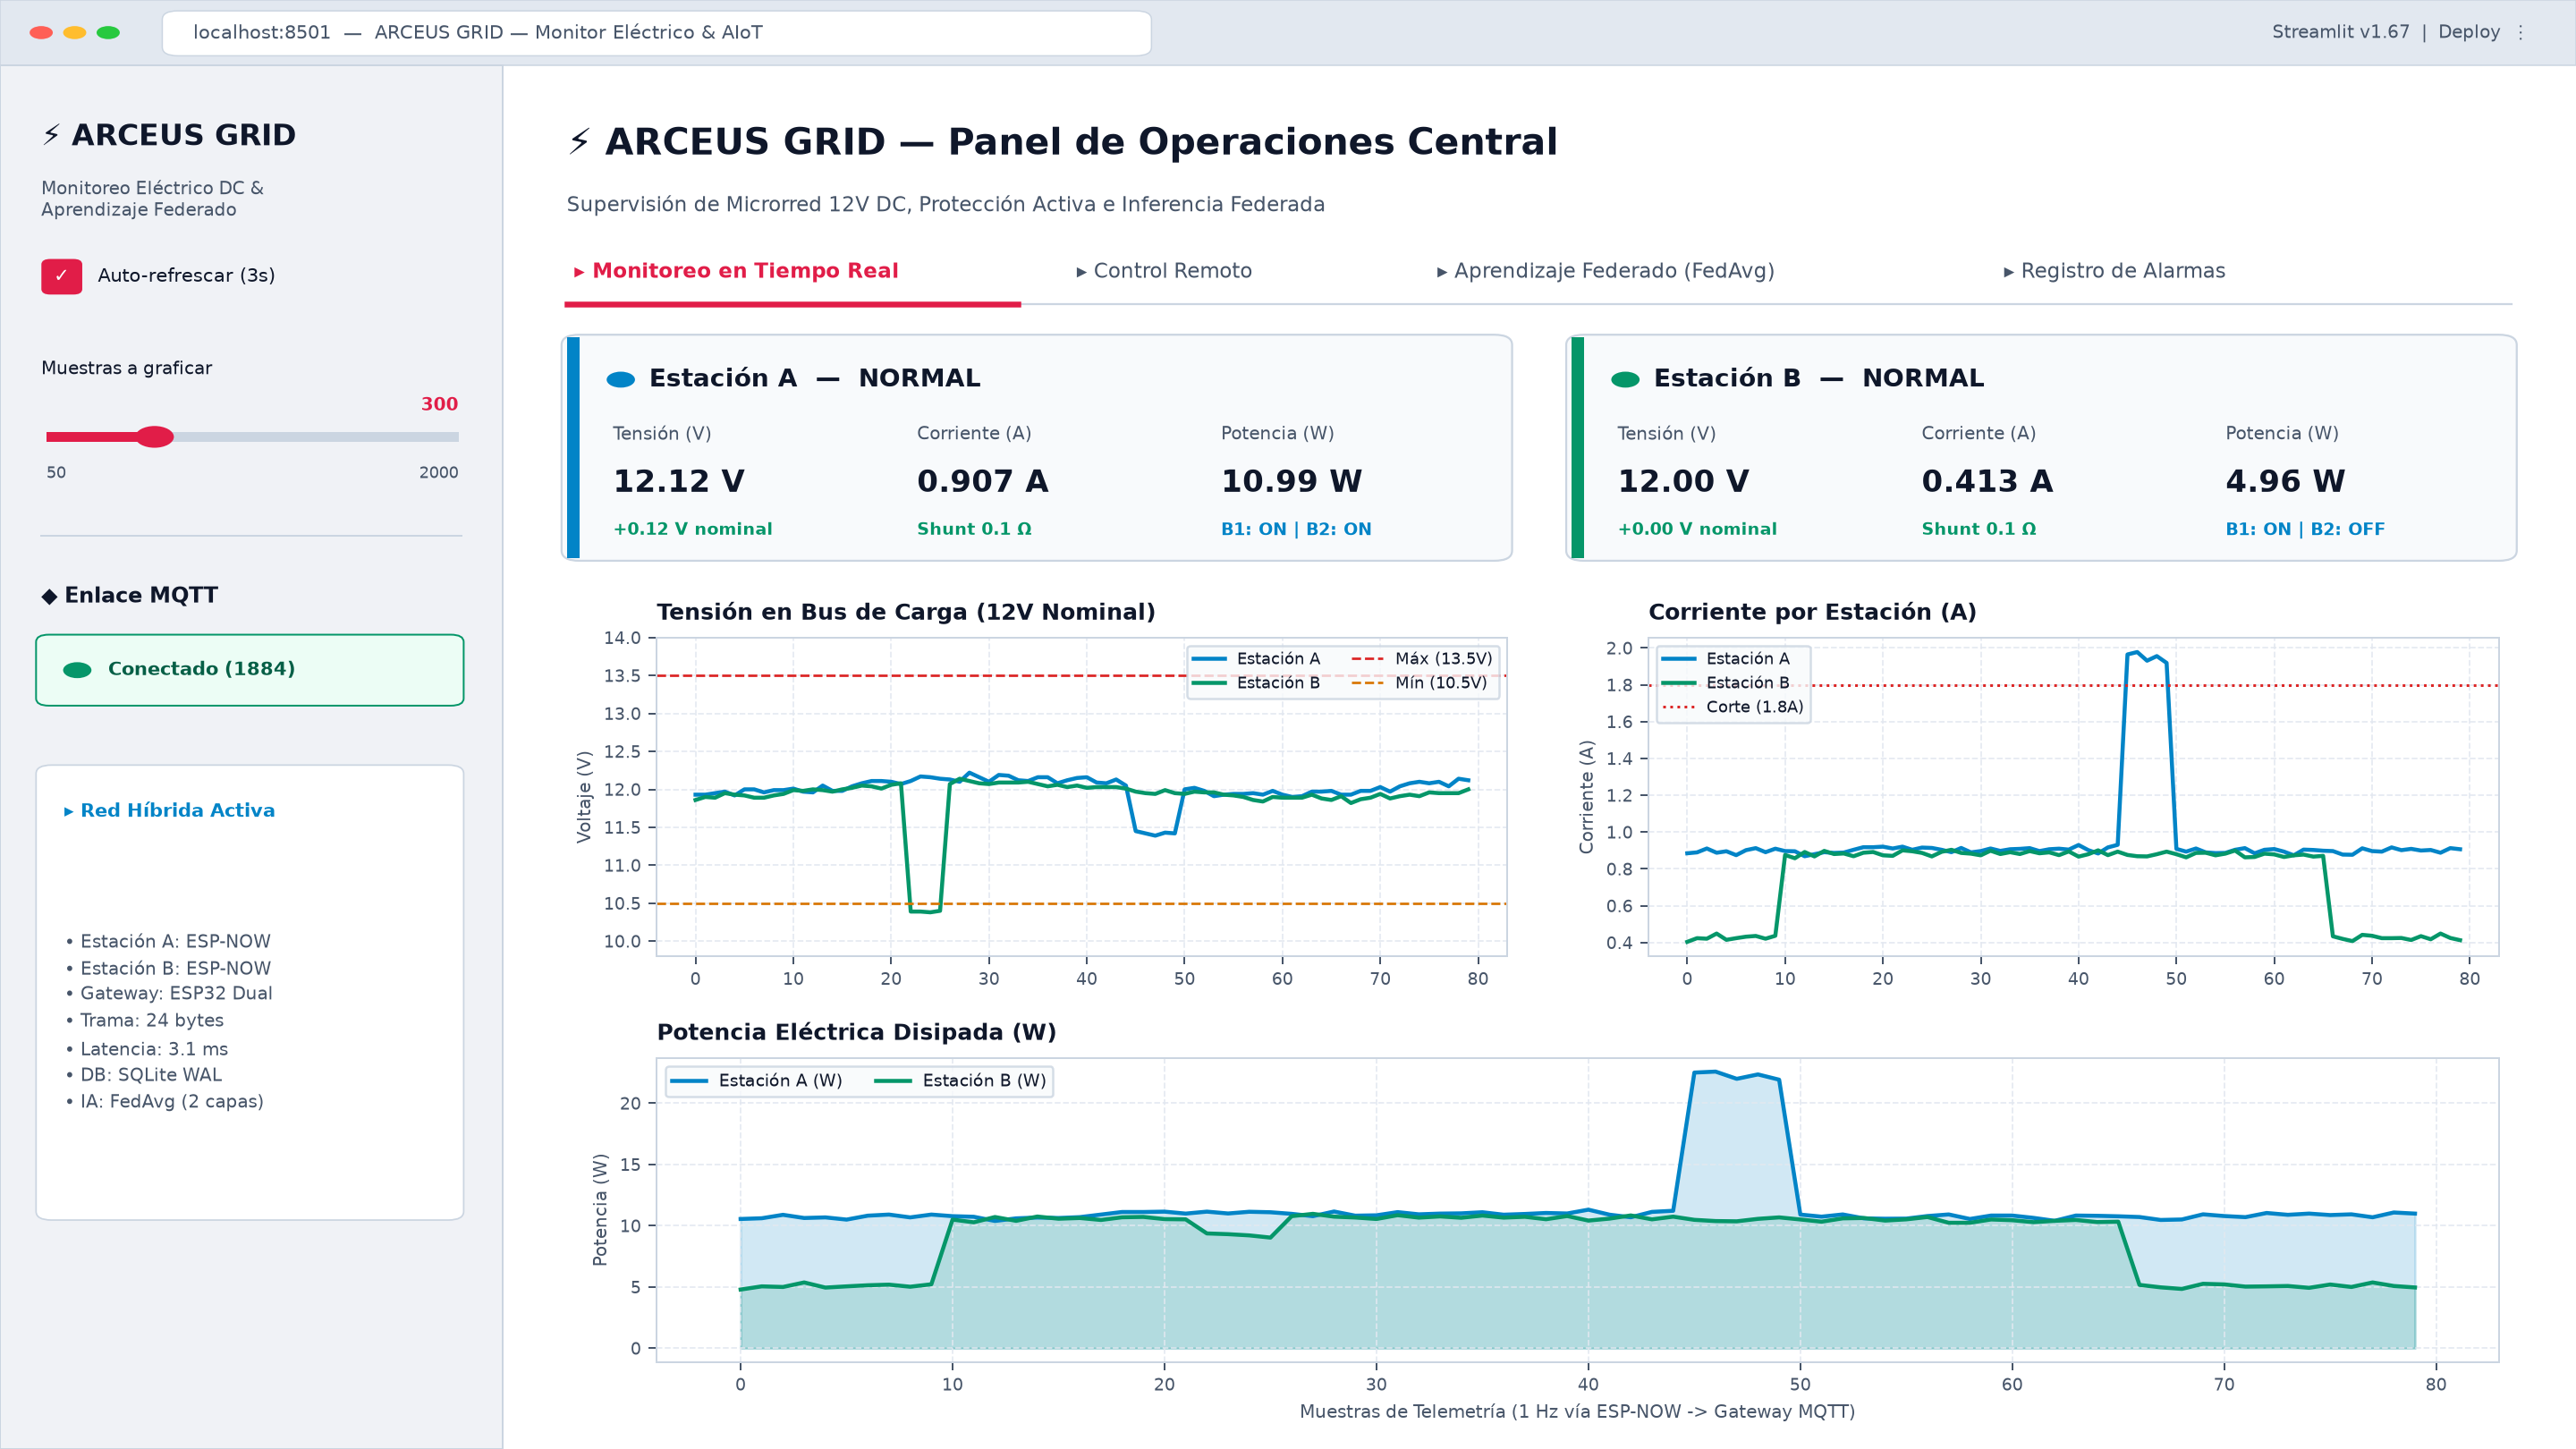
\includegraphics[width=0.96\linewidth]{figuras/interfaz_monitoreo.png}
    \end{column}
  \end{columns}
\end{frame}

% ==============================================================================
% 10. PROTECCIÓN ACTIVA Y DETECCIÓN DE ANOMALÍAS (Imagen + Regla 6x6)
% ==============================================================================
\begin{frame}{8. Detección de Anomalías y Corte}{Protección en el Borde y Puntaje Estadístico Z-Score}
  \vspace{0.1cm}
  \begin{columns}[c,onlytextwidth]
    \begin{column}{0.38\textwidth}
      \small
      \begin{itemize}\setlength{\itemsep}{8pt}
        \item \textbf{Sobrecorriente $>1.80\text{ A}$:} corte inmediato.
        \item \textbf{Subtensión $<10.50\text{ V}$:} alerta amarilla.
        \item \textbf{Anomalía estadística:}
          \[
            Z_V = \frac{|V - 12.0|}{0.35} > 3.0
          \]
      \end{itemize}
    \end{column}
    \begin{column}{0.60\textwidth}
      \centering
      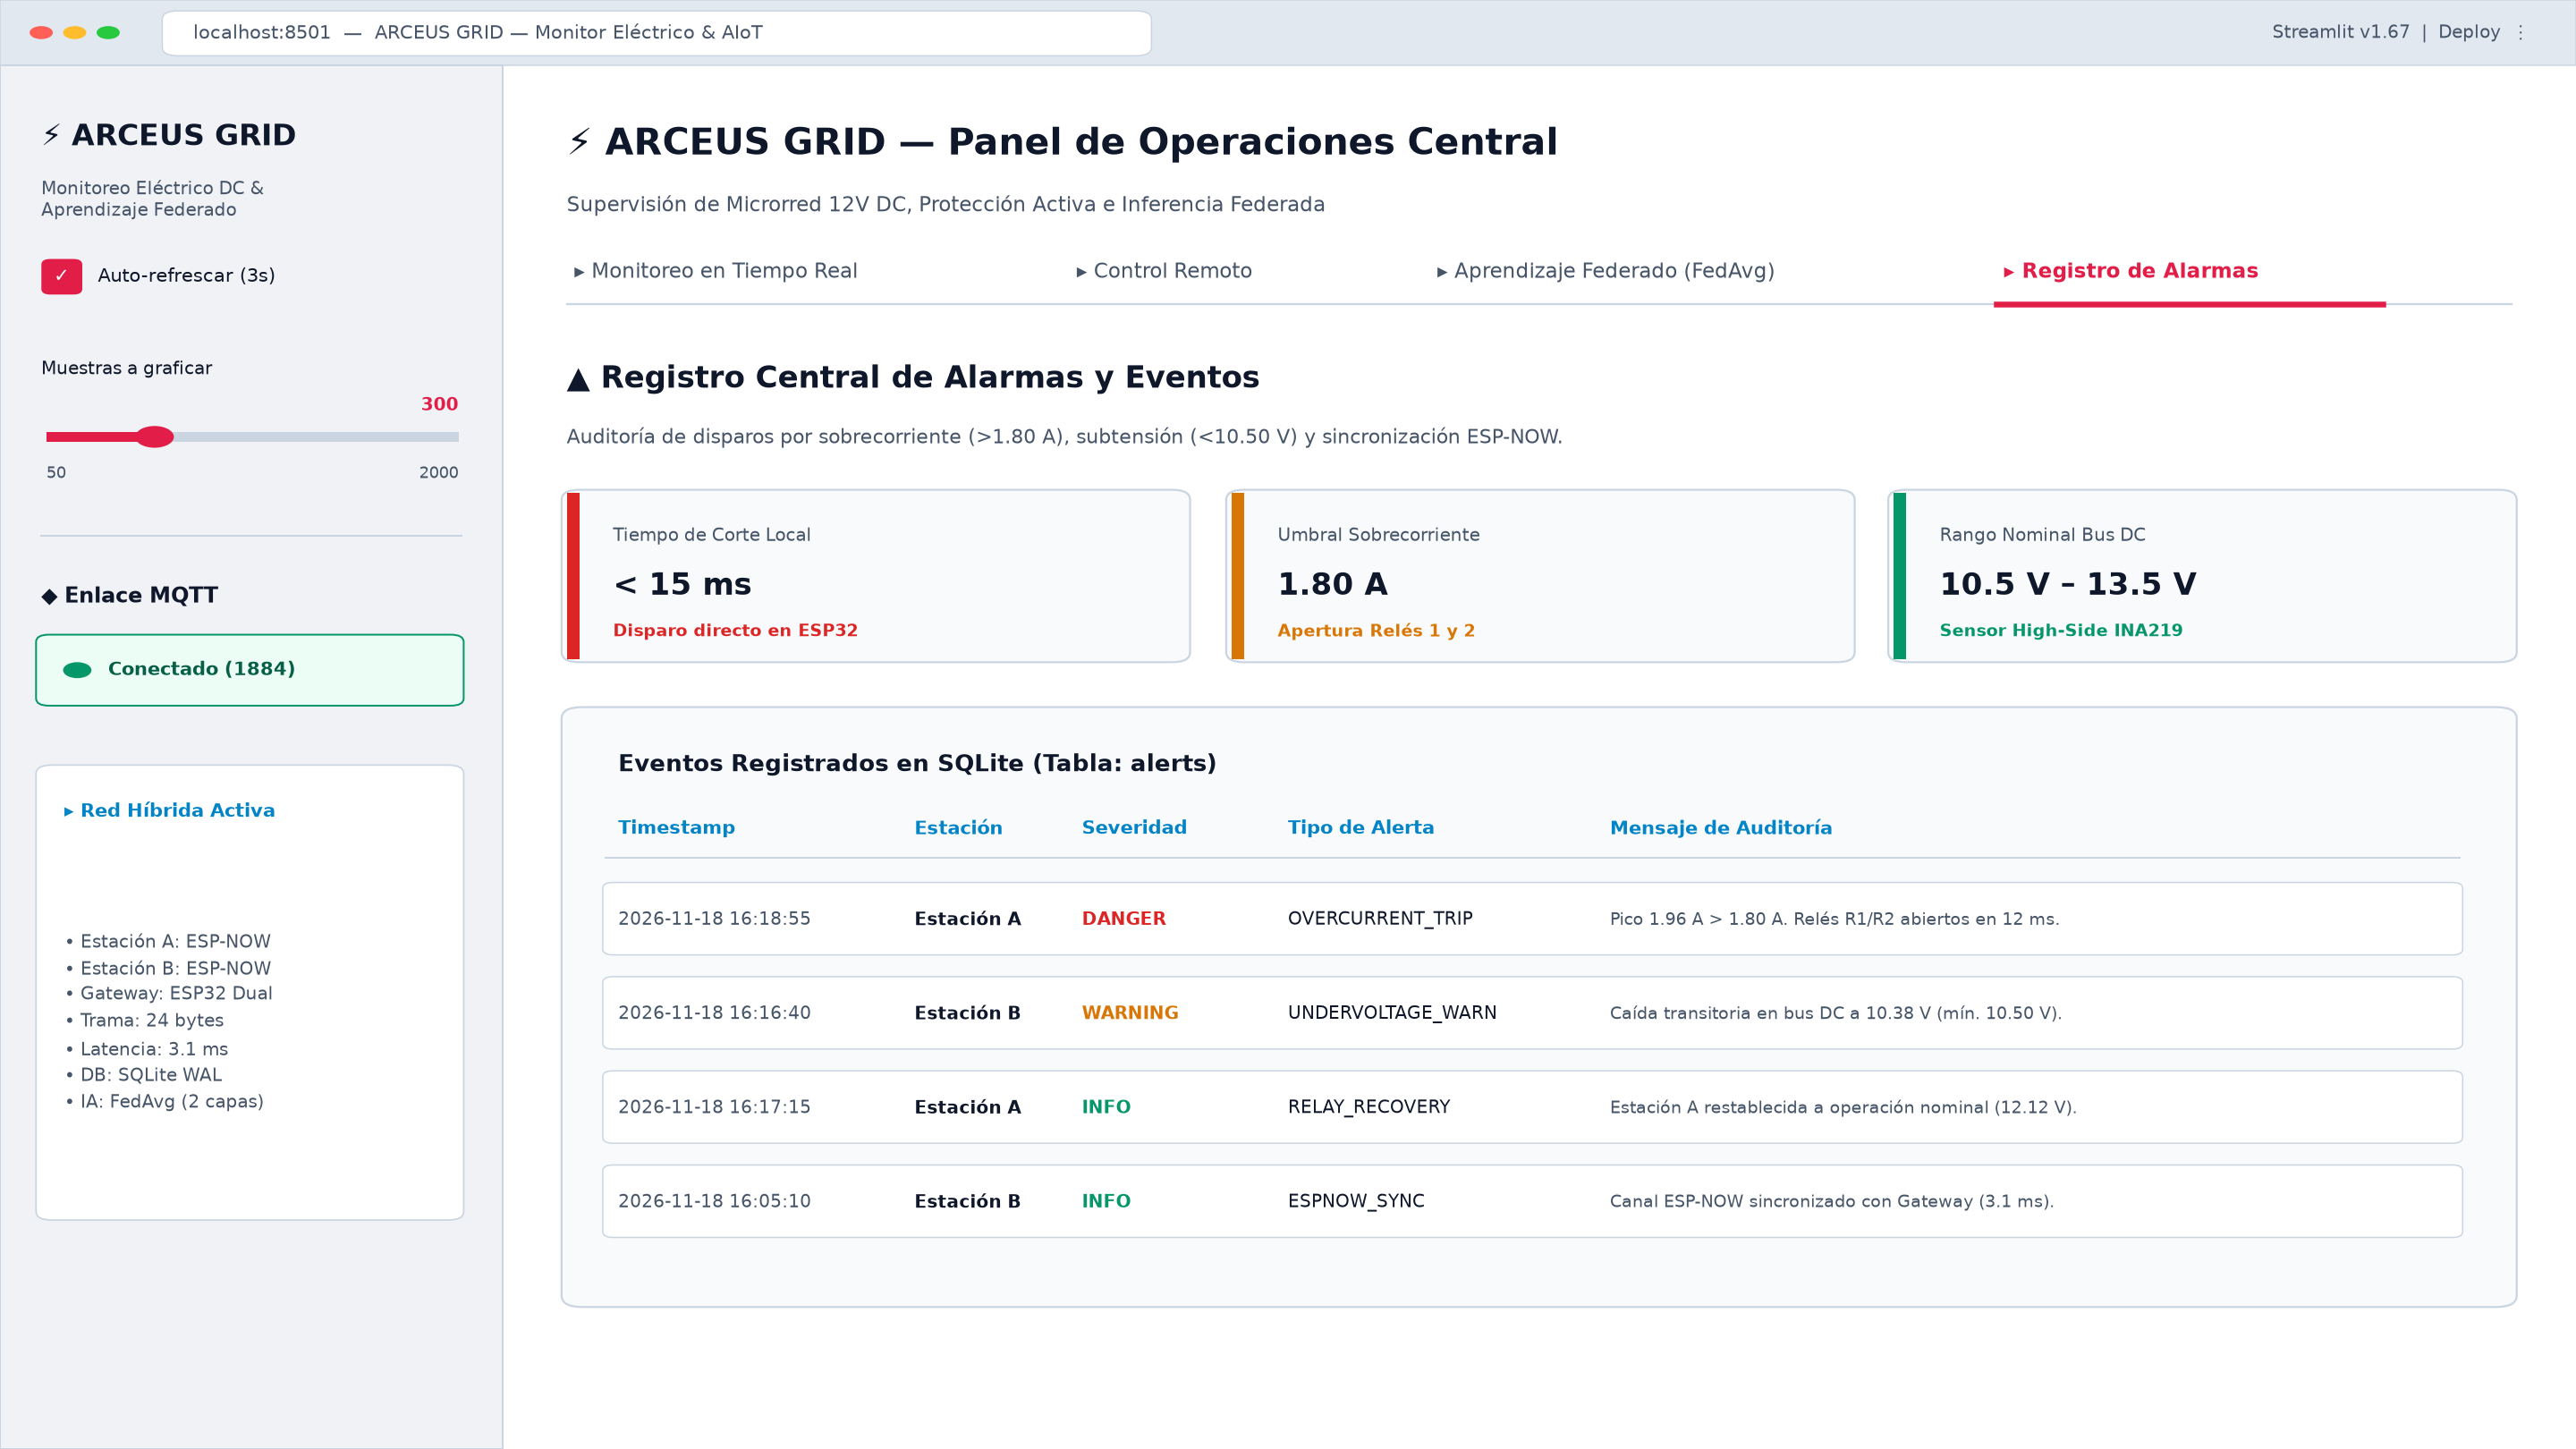
\includegraphics[width=0.96\linewidth]{figuras/interfaz_alarmas.png}
    \end{column}
  \end{columns}
\end{frame}

% ==============================================================================
% 11. APRENDIZAJE FEDERADO (FEDAVG) (Imagen + Fórmula Limpia + 3 Viñetas)
% ==============================================================================
\begin{frame}{9. Inteligencia Artificial: Algoritmo FedAvg}{Las Estaciones Aprenden sin Compartir Datos Crudos}
  \vspace{0.1cm}
  \begin{columns}[c,onlytextwidth]
    \begin{column}{0.38\textwidth}
      \small
      \begin{itemize}\setlength{\itemsep}{7pt}
        \item \textbf{Red local MLP} ($3 \rightarrow 8 \rightarrow 1$).
        \item \textbf{Solo viajan pesos} $(\mathbf{W}, \mathbf{b})$.
        \item \textbf{95\% menos tráfico} en la red.
      \end{itemize}
      \vspace{0.05cm}
      \begin{softcard}[brandblue]{\faBrain\ Promedio Federado}
        \centering\footnotesize
        \[
          \theta_{t+1}^{\text{global}} = \sum_{k \in \{A,B\}} \frac{n_k}{N}\,\theta_{t+1}^k
        \]
      \end{softcard}
    \end{column}
    \begin{column}{0.60\textwidth}
      \centering
      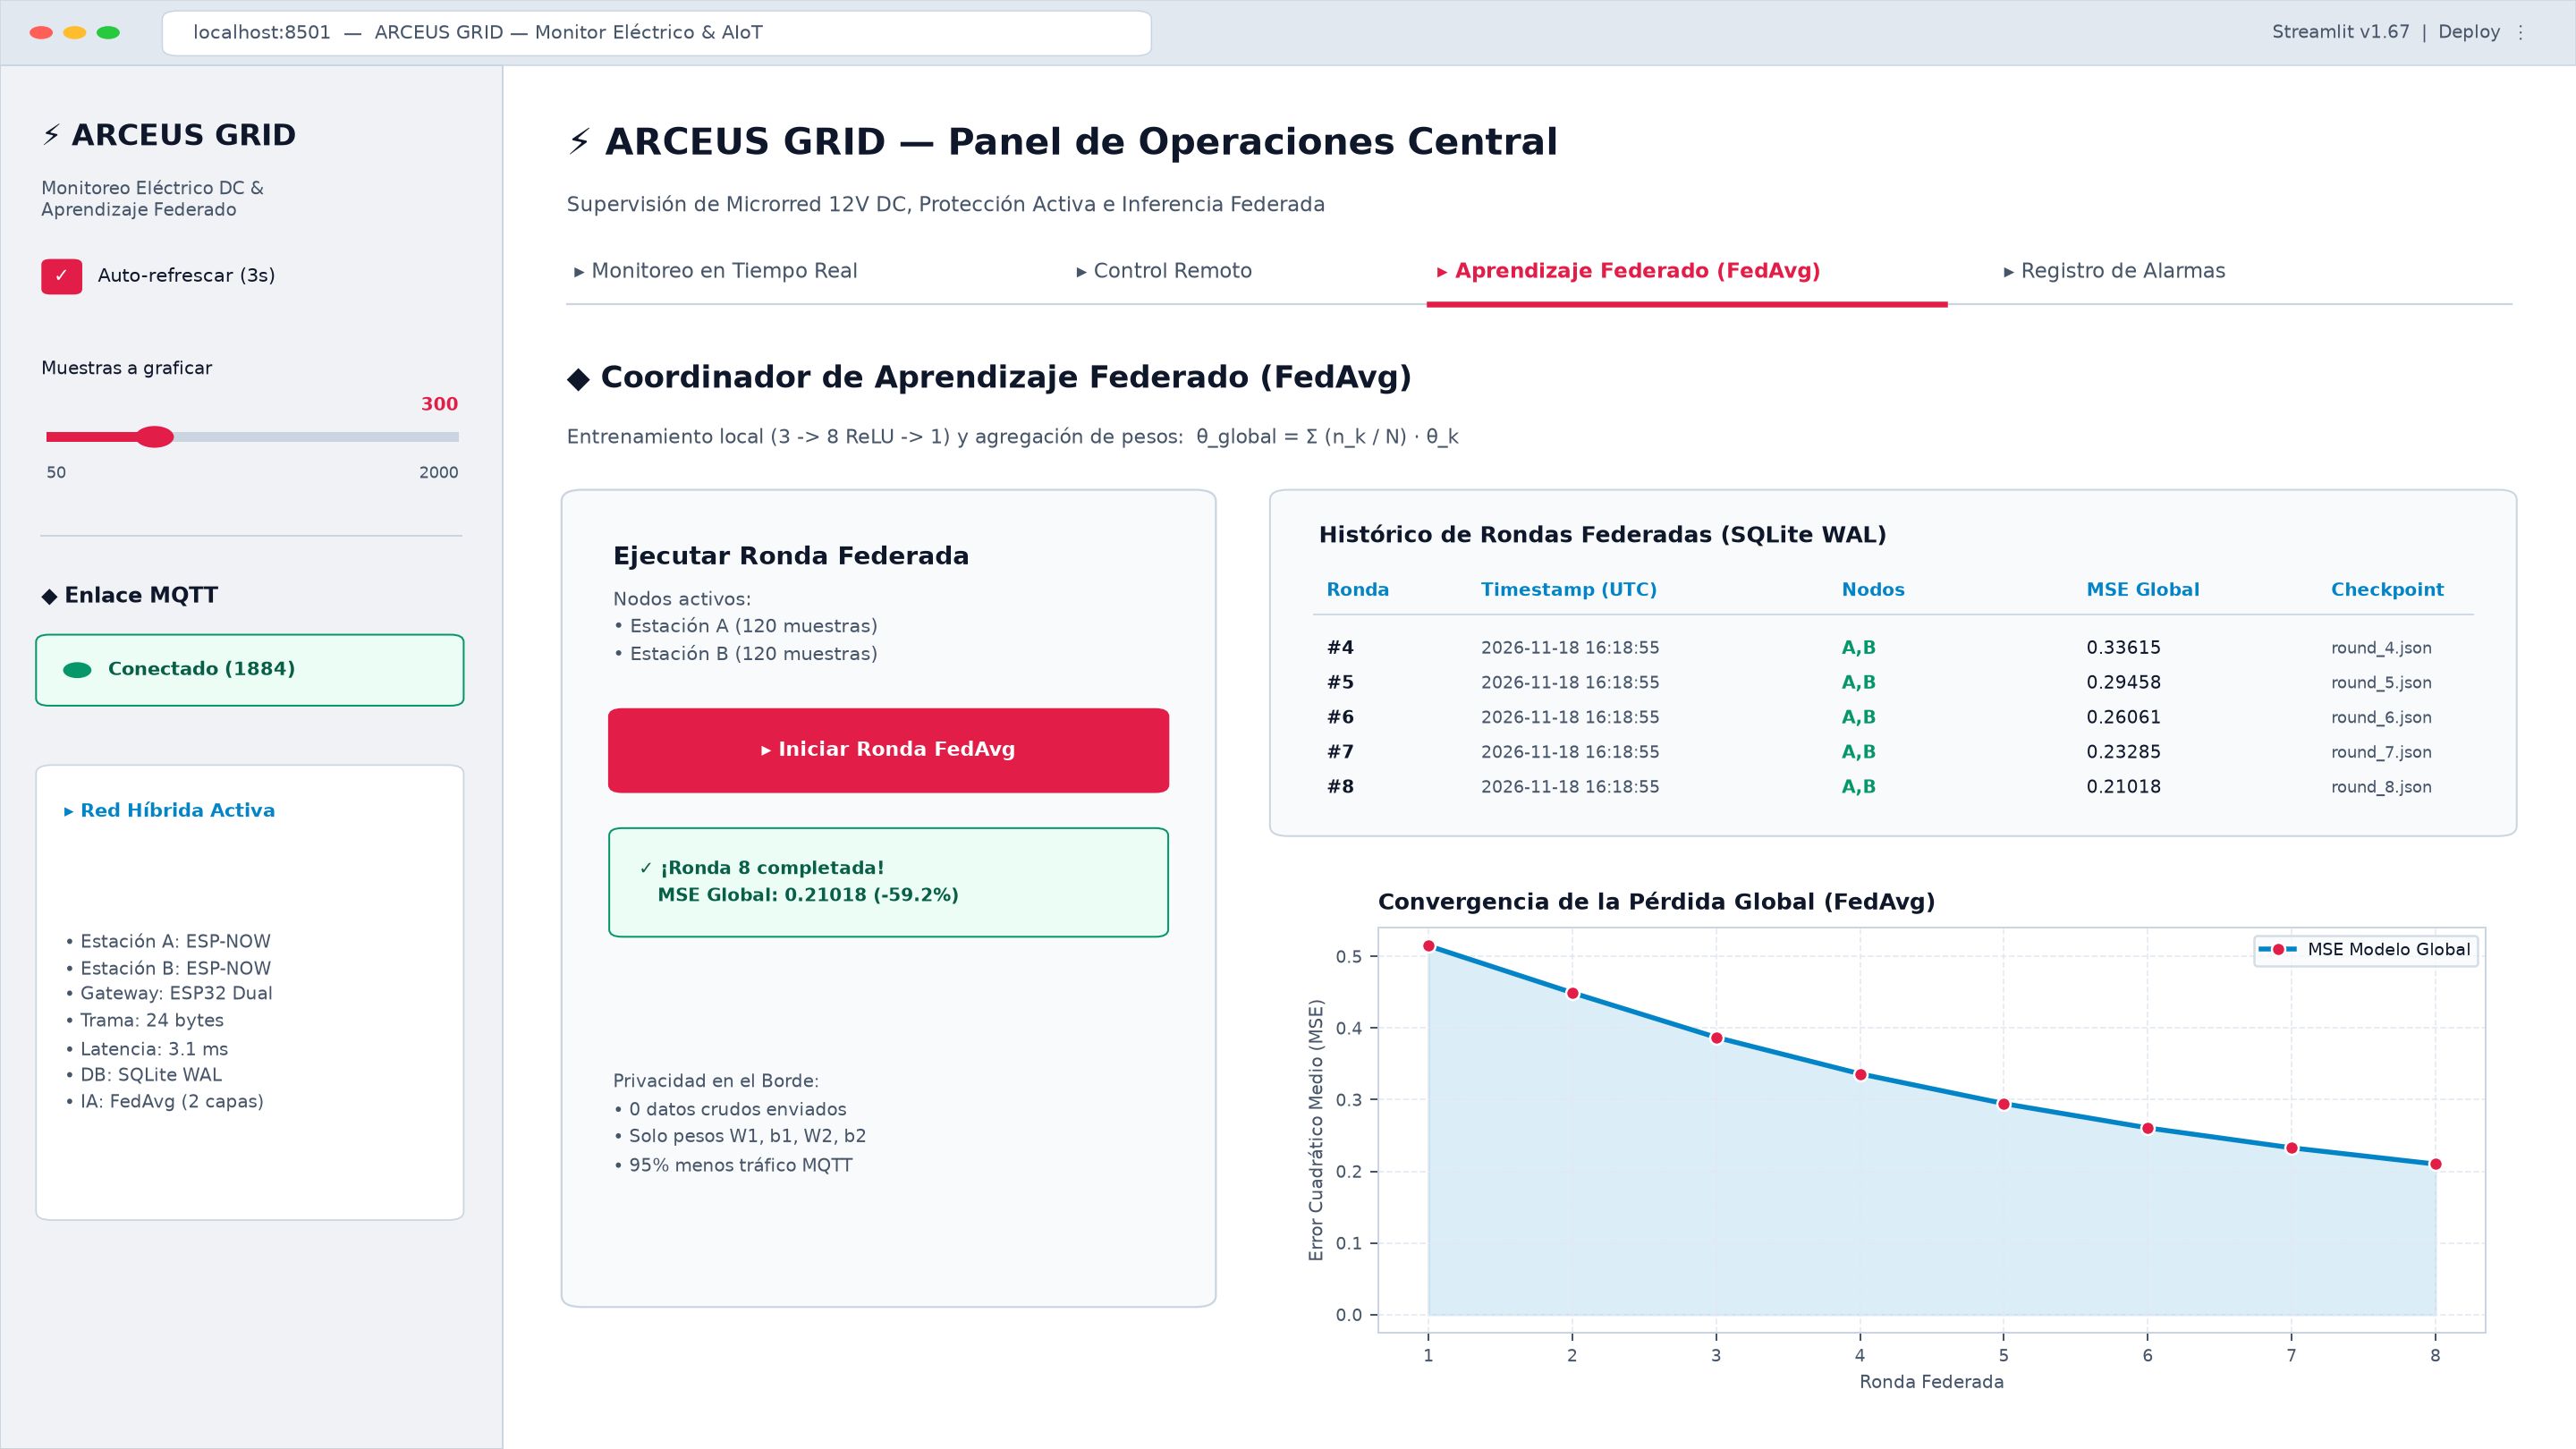
\includegraphics[width=0.96\linewidth]{figuras/interfaz_fedavg.png}
    \end{column}
  \end{columns}
\end{frame}

% ==============================================================================
% 12. CONTROL REMOTO Y RESULTADOS (Imagen + 4 Métricas Puntuales)
% ==============================================================================
\begin{frame}{10. Control Remoto y Resultados}{Desempeño Experimental Validado en Laboratorio}
  \vspace{0.1cm}
  \begin{columns}[c,onlytextwidth]
    \begin{column}{0.38\textwidth}
      \normalsize
      \begin{itemize}\setlength{\itemsep}{9pt}
        \item \textbf{Corte local:} $< 15\text{ ms}$.
        \item \textbf{Latencia radio:} $\approx 3.2\text{ ms}$.
        \item \textbf{Reducción MSE:} $-59.2\%$.
        \item \textbf{Reinicios por ruido:} $0$.
      \end{itemize}
    \end{column}
    \begin{column}{0.60\textwidth}
      \centering
      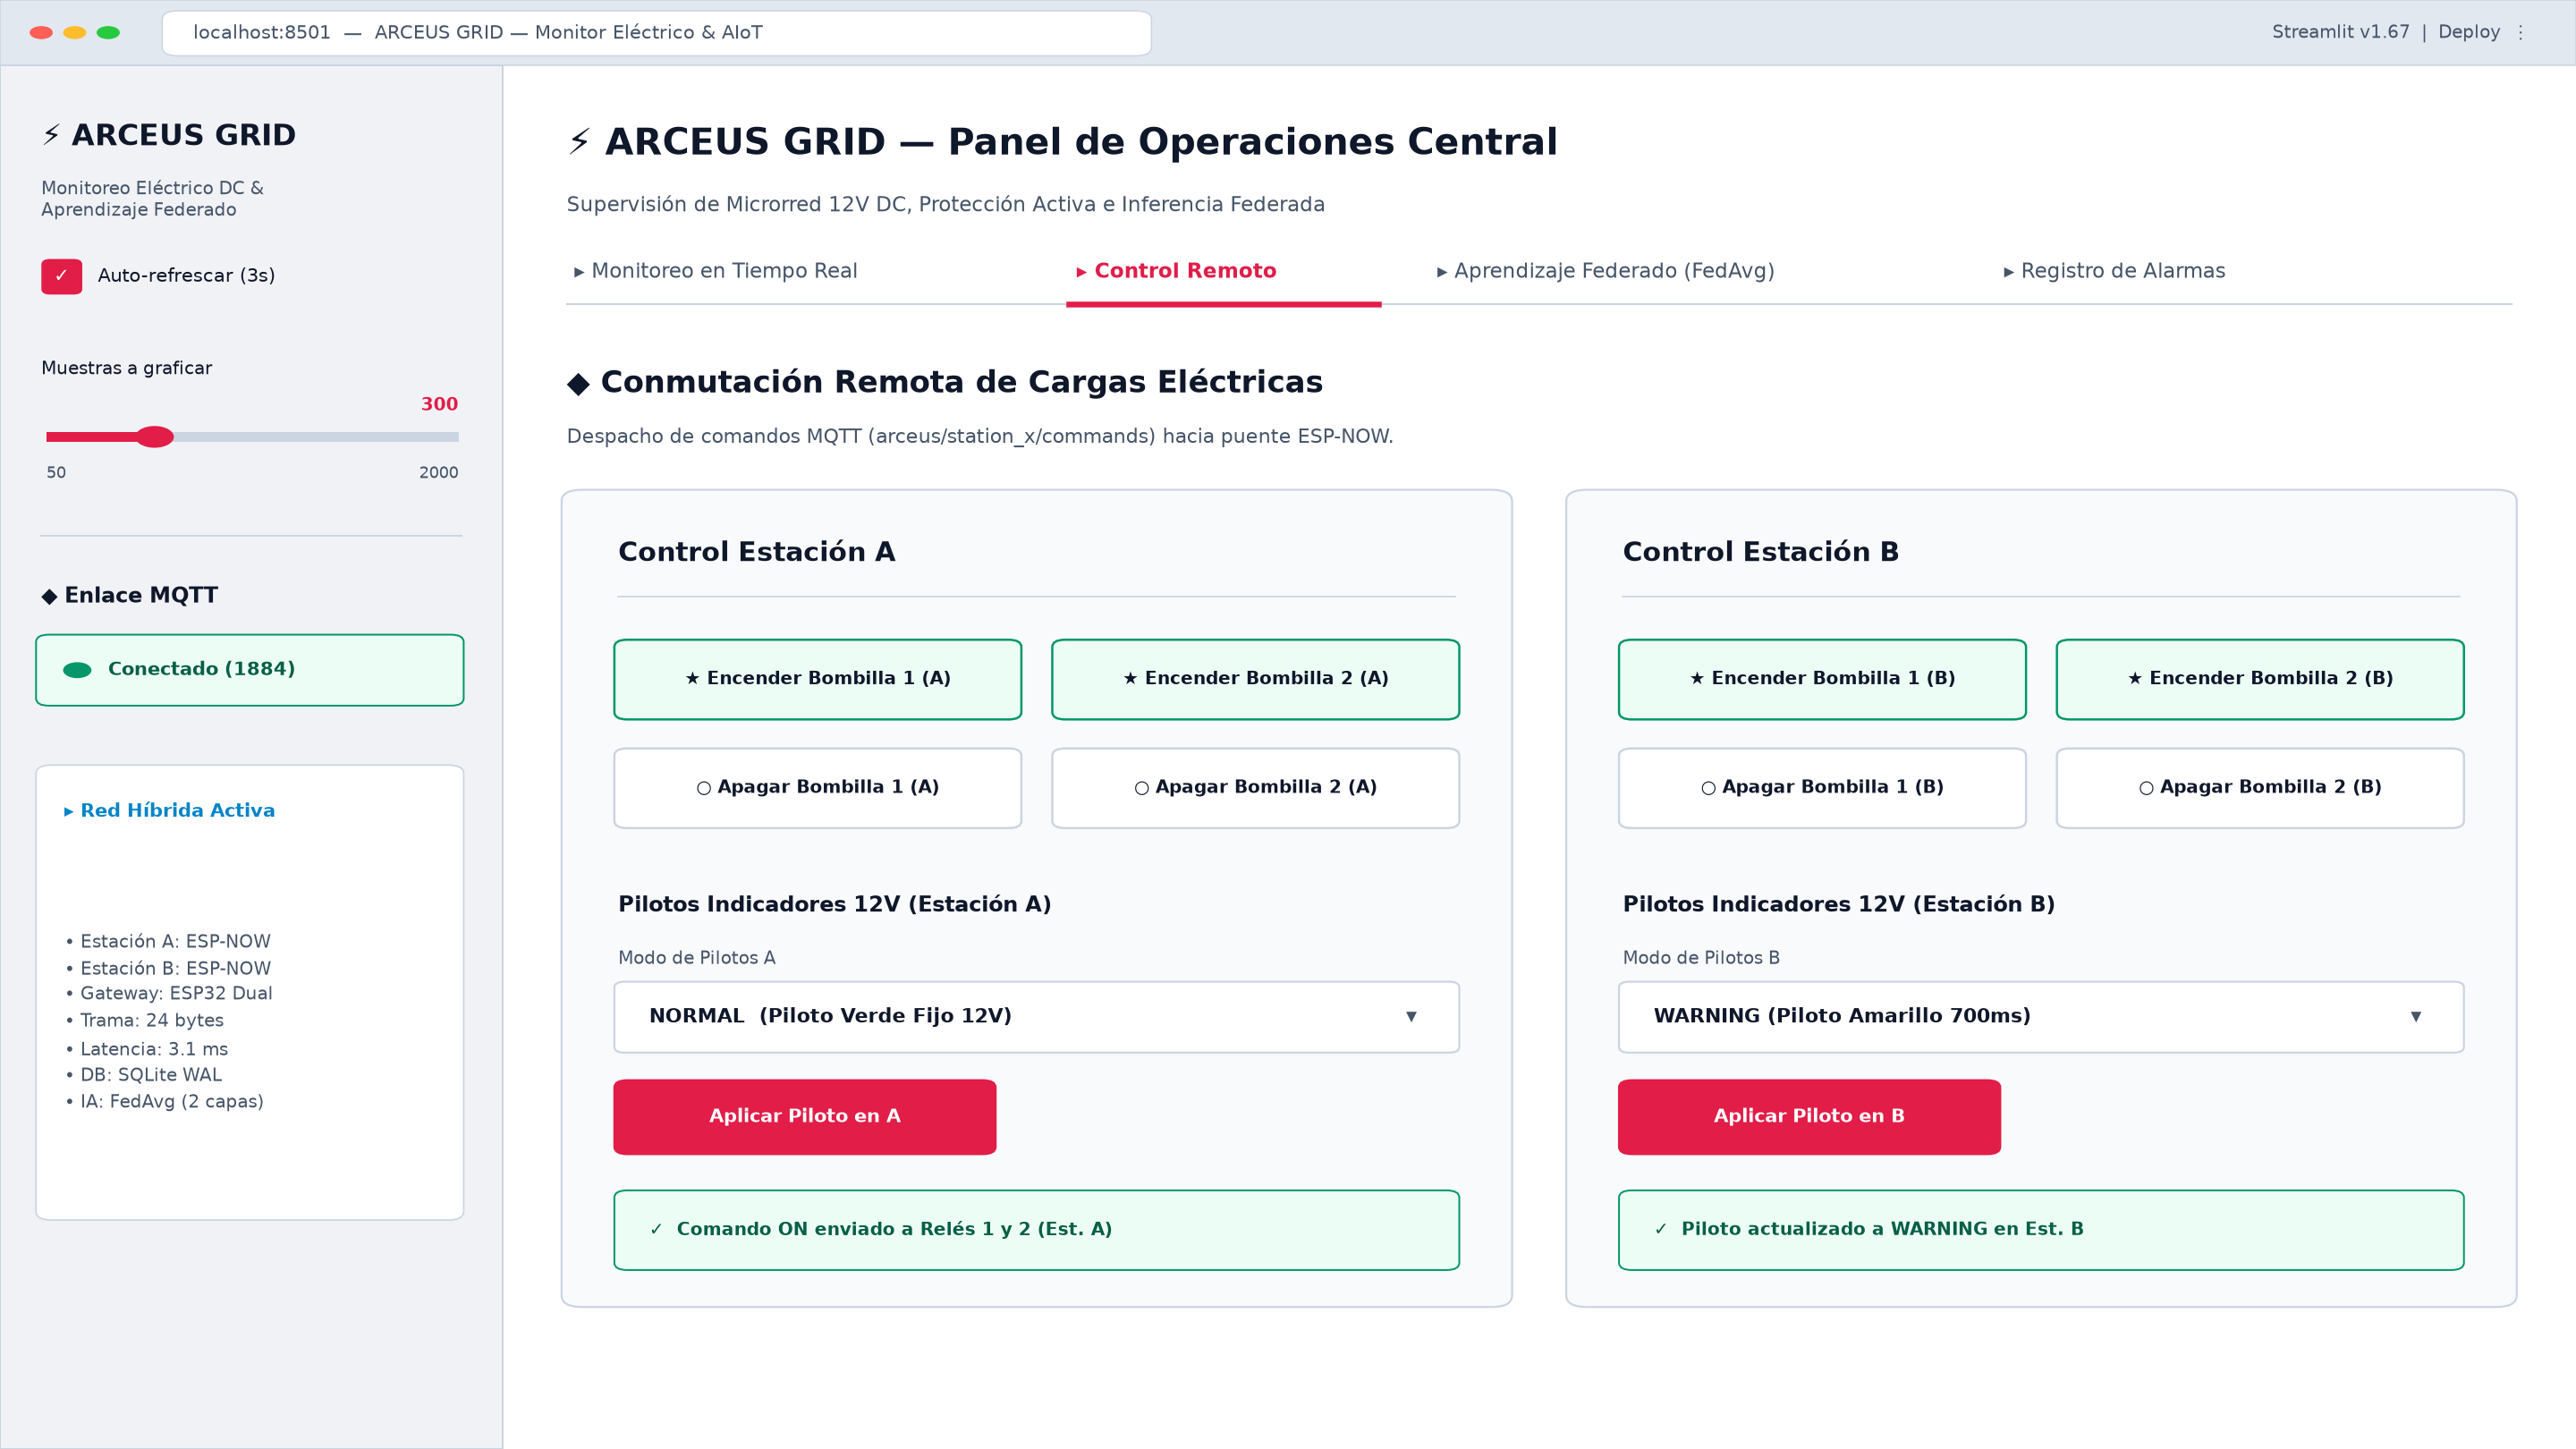
\includegraphics[width=0.96\linewidth]{figuras/interfaz_control.png}
    \end{column}
  \end{columns}
\end{frame}

% ==============================================================================
% 13. CONCLUSIONES (Guía: Cierre claro + llamada a la acción / futuro)
% ==============================================================================
\begin{frame}{11. Conclusiones y Próximos Pasos}{Síntesis del Impacto Técnico}
  \vspace{0.15cm}
  \begin{columns}[c,onlytextwidth]
    \begin{column}{0.55\textwidth}
      \normalsize
      \begin{itemize}\setlength{\itemsep}{10pt}
        \item \textbf{Aislamiento JD-VCC} eliminó fallas eléctricas.
        \item \textbf{ESP-NOW + MQTT} desacopló los sensores.
        \item \textbf{FedAvg} entrenó con privacidad total.
        \item \textbf{Futuro:} PCB KiCad, TinyML y Solar.
      \end{itemize}
    \end{column}
    \begin{column}{0.41\textwidth}
      \begin{softcard}[brandgreen]{\faCheckDouble\ Mensaje Clave}
        \small
        \textbf{ARCEUS GRID} demuestra que es posible proteger y entrenar microrredes inteligentes en tiempo real con hardware accesible.
      \end{softcard}
    \end{column}
  \end{columns}
\end{frame}

% ==============================================================================
% 14. CIERRE (Estilo Página 10 de la guía: ¡Muchas gracias por su atención!)
% ==============================================================================
\begin{frame}[plain]
  \begin{tikzpicture}[remember picture,overlay]
    \fill[brandblue!12] (current page.north west) -- ++(4.2,0) -- ++(-4.2,-2.6) -- cycle;
    \fill[brandgreen!12] (current page.south east) -- ++(-4.5,0) -- ++(4.5,2.8) -- cycle;
    \fill[brandamber!15] ($(current page.north east)+(-2.2,-1.1)$) circle (0.9cm);
    \fill[brandblue!10] ($(current page.south west)+(2.0,1.0)$) circle (0.7cm);
  \end{tikzpicture}

  \vspace{1.5cm}
  \begin{center}
    {\Huge\bfseries\color{inkdark}¡MUCHAS GRACIAS}\\[8pt]
    {\Huge\bfseries\color{brandblue}POR SU ATENCIÓN!}\\[18pt]
    {\large\color{inkmuted}¿Preguntas o comentarios del jurado?}\\[14pt]
    \begin{tikzpicture}
      \node[fill=bgsoft,draw=brandblue!40,line width=0.8pt,rounded corners=4pt,
            inner xsep=14pt,inner ysep=6pt,font=\small\bfseries,text=inkdark]
        {Owen Mora $\cdot$ Angelo Charris $\cdot$ Braulio Ribón $\cdot$ Manuel Pertuz $\cdot$ Milton Sánchez};
    \end{tikzpicture}
  \end{center}
\end{frame}

\end{document}
